\documentclass[aspectratio=169]{beamer}
\usepackage{ulem}
\usepackage{tikz}
\usepackage{booktabs}
 \usepackage{graphicx,threeparttable,caption}
\usetikzlibrary{shapes,snakes}
\usepackage[beamer,customcolors]{hf-tikz}
\usepackage{nicematrix}
\usepackage{xcolor}
\usepackage{makecell}
\usepackage{array}
\usepackage{csquotes}
\usepackage{csquotes}
\usepackage{minted}
\captionsetup{labelformat=empty,labelsep=none}

\graphicspath{ {./png/} }

\usetikzlibrary{
    arrows,
    arrows.meta,
    shapes,
    positioning,
    shadows,
    trees,
    calc
}

\tikzset{%
    >={Latex[width=2mm,length=2mm]},
    % Specifications for style of nodes:
    plain/.style = {},
    base/.style = {
        plain,
        rectangle, rounded corners, draw=black,
        minimum width=1cm, minimum height=1cm,
        text centered, font=\sffamily\tiny\bfseries,
        fill=white, align=center
    },
    app/.style = {base, ellipse},
    data/.style = {base, fill=gray!30},
    action/.style = {base, circle, fill=red!30},
    note/.style = {app, fill=yellow},
    hl/.style={
    set fill color=red!80!black!40,
    set border color=red!80!black
    }
}


\AtBeginSection[]{
  \begin{frame}
  \vfill
  \centering
  \begin{beamercolorbox}[sep=8pt,center,shadow=true,rounded=true]{title}
    \usebeamerfont{title}\insertsectionhead\par%
  \end{beamercolorbox}
  \vfill
  \end{frame}
}
%\usecolortheme[orchid]{structure}
\usetheme[hideothersubsections]{PaloAlto}
\makeatletter
\patchcmd{\csq@bquote@i}{{#6}}{{\emph{#6}}}{}{}
\makeatother
%\usecolortheme{orchid}
%\usefonttheme{professionalfonts}
\newcommand{\soutthick}[1]{%
   \textcolor{red}{
   \renewcommand{\ULthickness}{1pt}%
      \sout{#1}%
   \renewcommand{\ULthickness}{.4pt}% Resetting to ulem default
   }
}
\newcommand{\centered}[1]{\begin{tabular}{l} #1 \end{tabular}}
\setbeamertemplate{section in toc}[square]
\setbeamertemplate{subsection in toc}[square]
\setbeamertemplate{secion in sidebar}[shaded]
\setbeamertemplate{items}[square]
\setbeamercovered{transparent} 

\title[]{Introduction to Computational Social Science}
\subtitle{Digital data sources and where to find them}
\author[]{Mikołaj Biesaga\\ \small{\color{blue}{\href{mailto:m.biesaga@uw.edu.pl}{m.biesaga@uw.edu.pl}}}}
\institute{
\includegraphics[width = 4 cm]{uw.png}}
\date{\today}
\begin{document}
\begin{frame}
   \titlepage
\end{frame}

\section[Data]{Data}

\subsection[Data Sources]{Data Sources}
\begin{frame}
    \setbeamercovered{transparent}
    \frametitle{Data Sources}
    \only<+>{
        \begin{figure}
            
\includegraphics[scale=.35]{png/data_everywhere.png}
        \end{figure}}
    \only<+>{
        \begin{figure}
            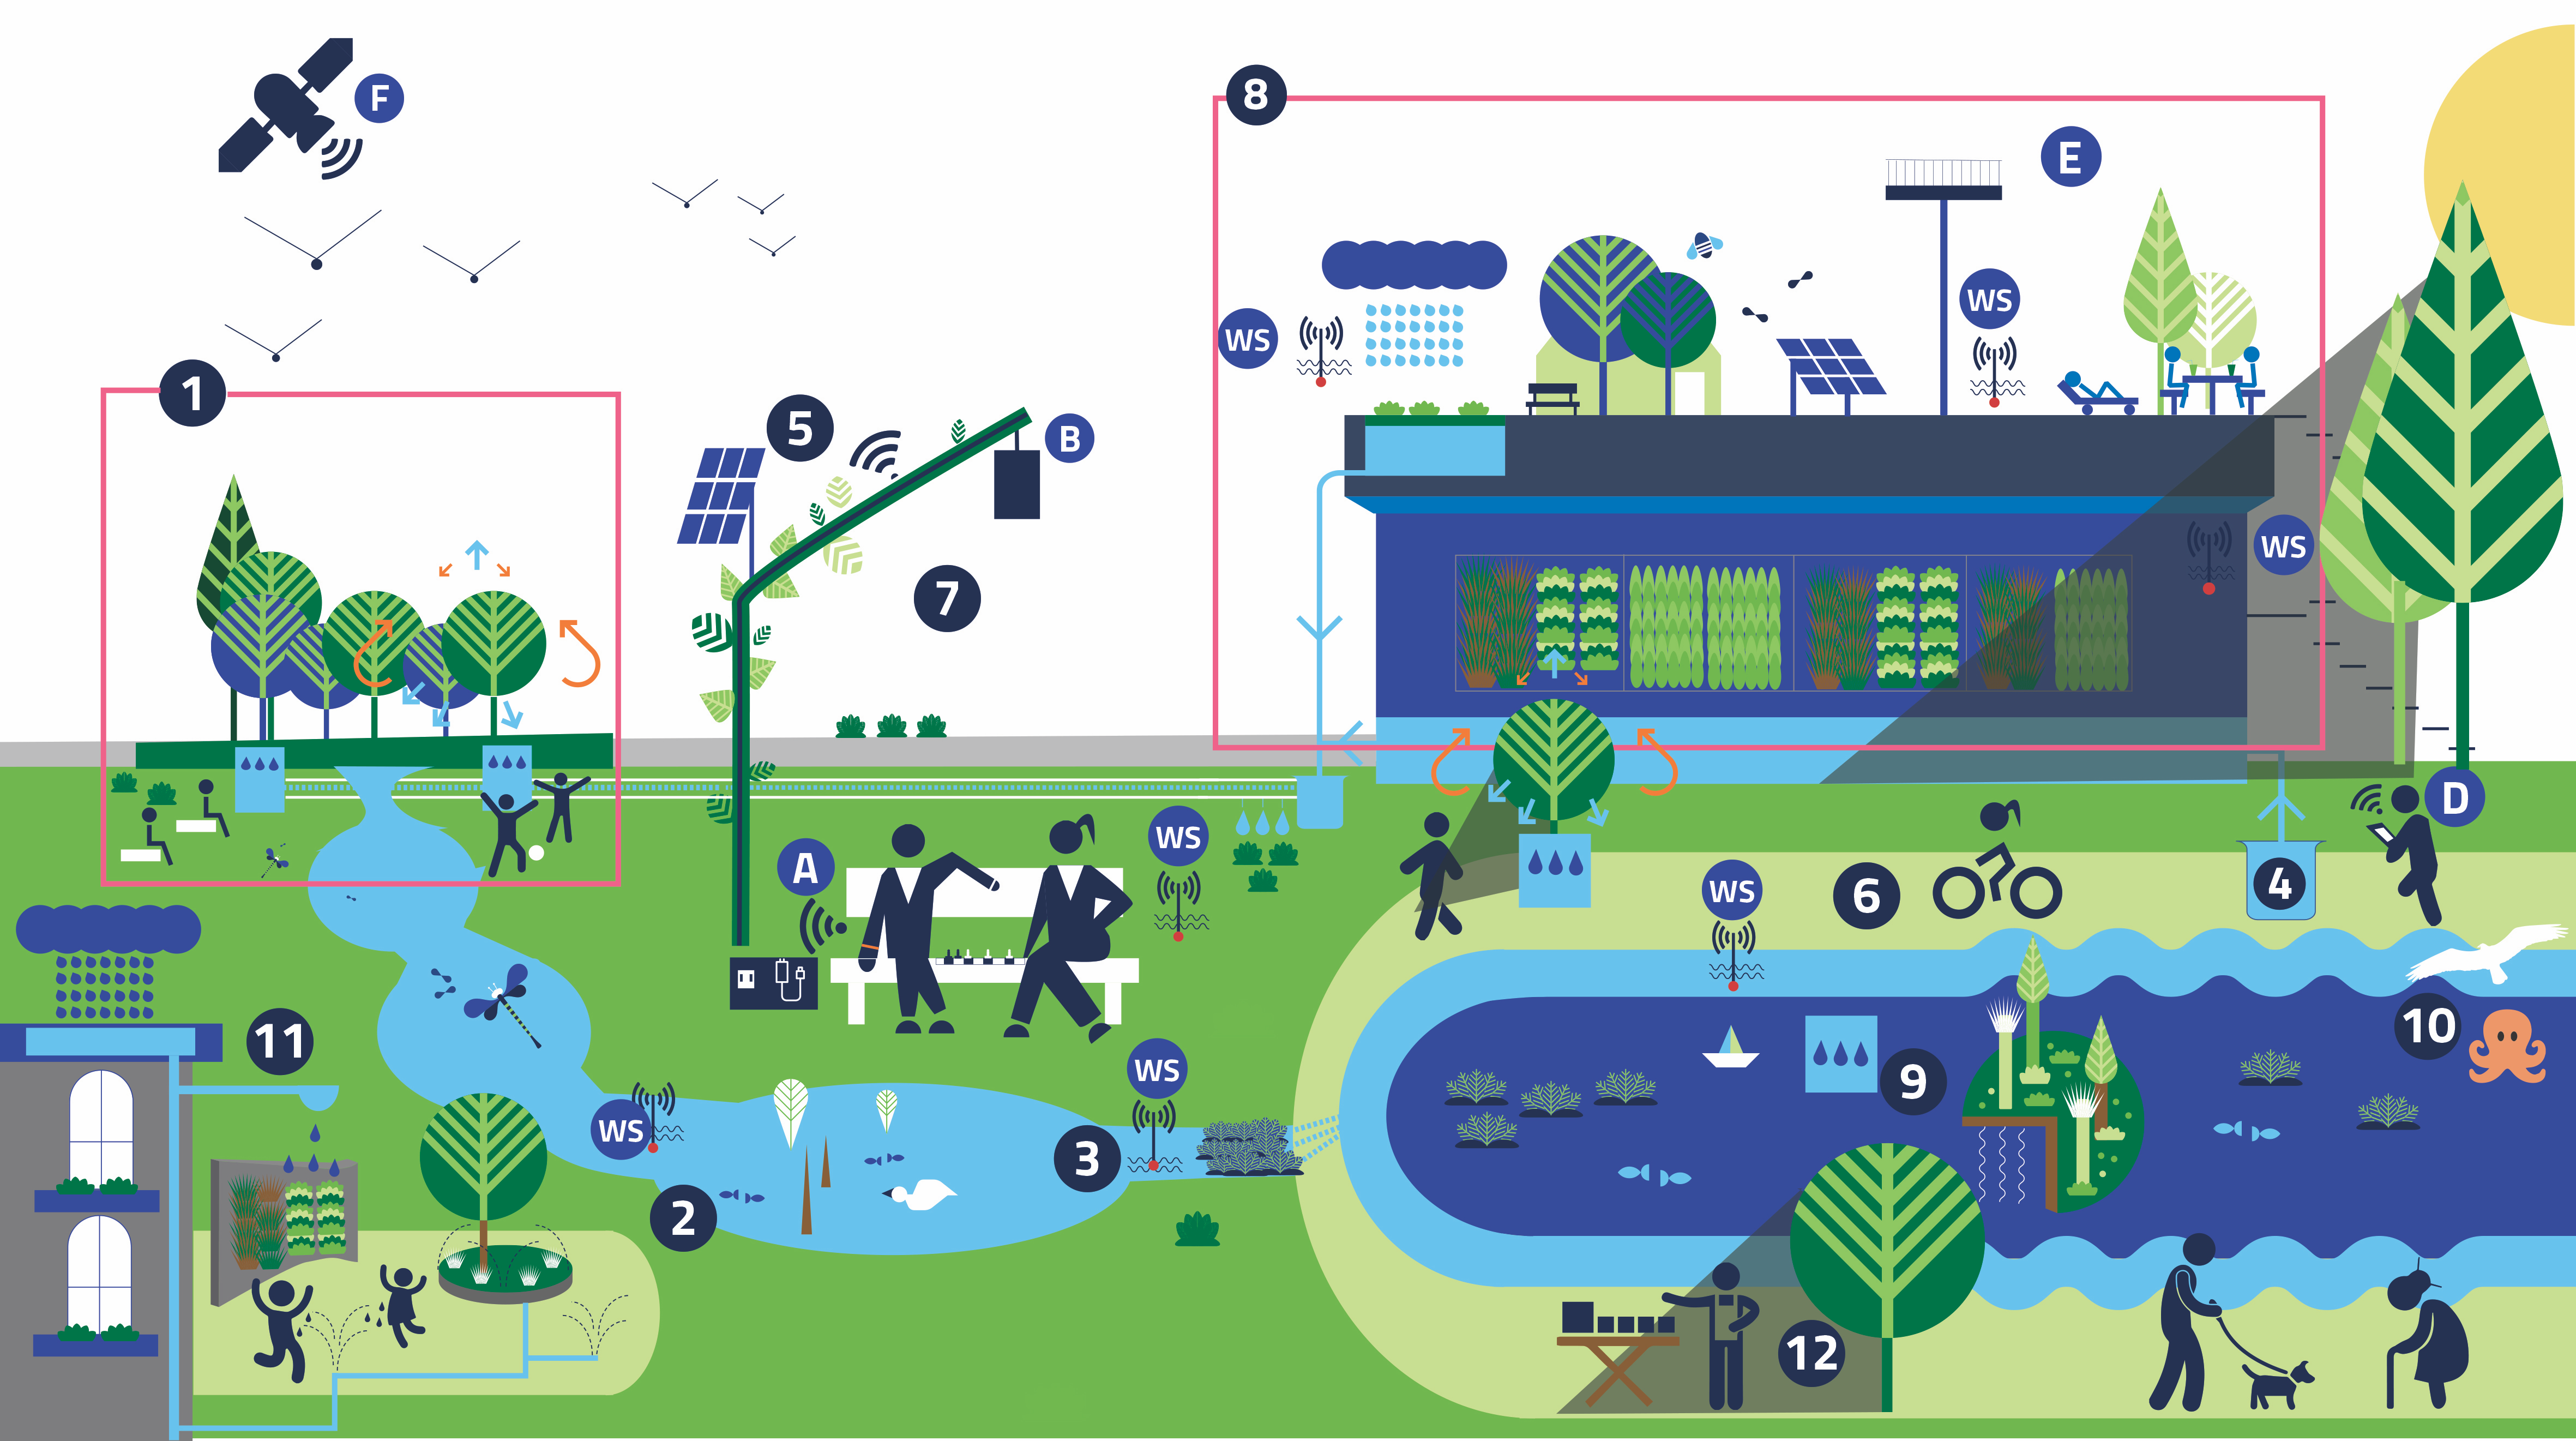
\includegraphics[width = .8\textwidth]{png/mierzenie.png}
        \end{figure}
    }
    \only<+>{
        \begin{figure}
            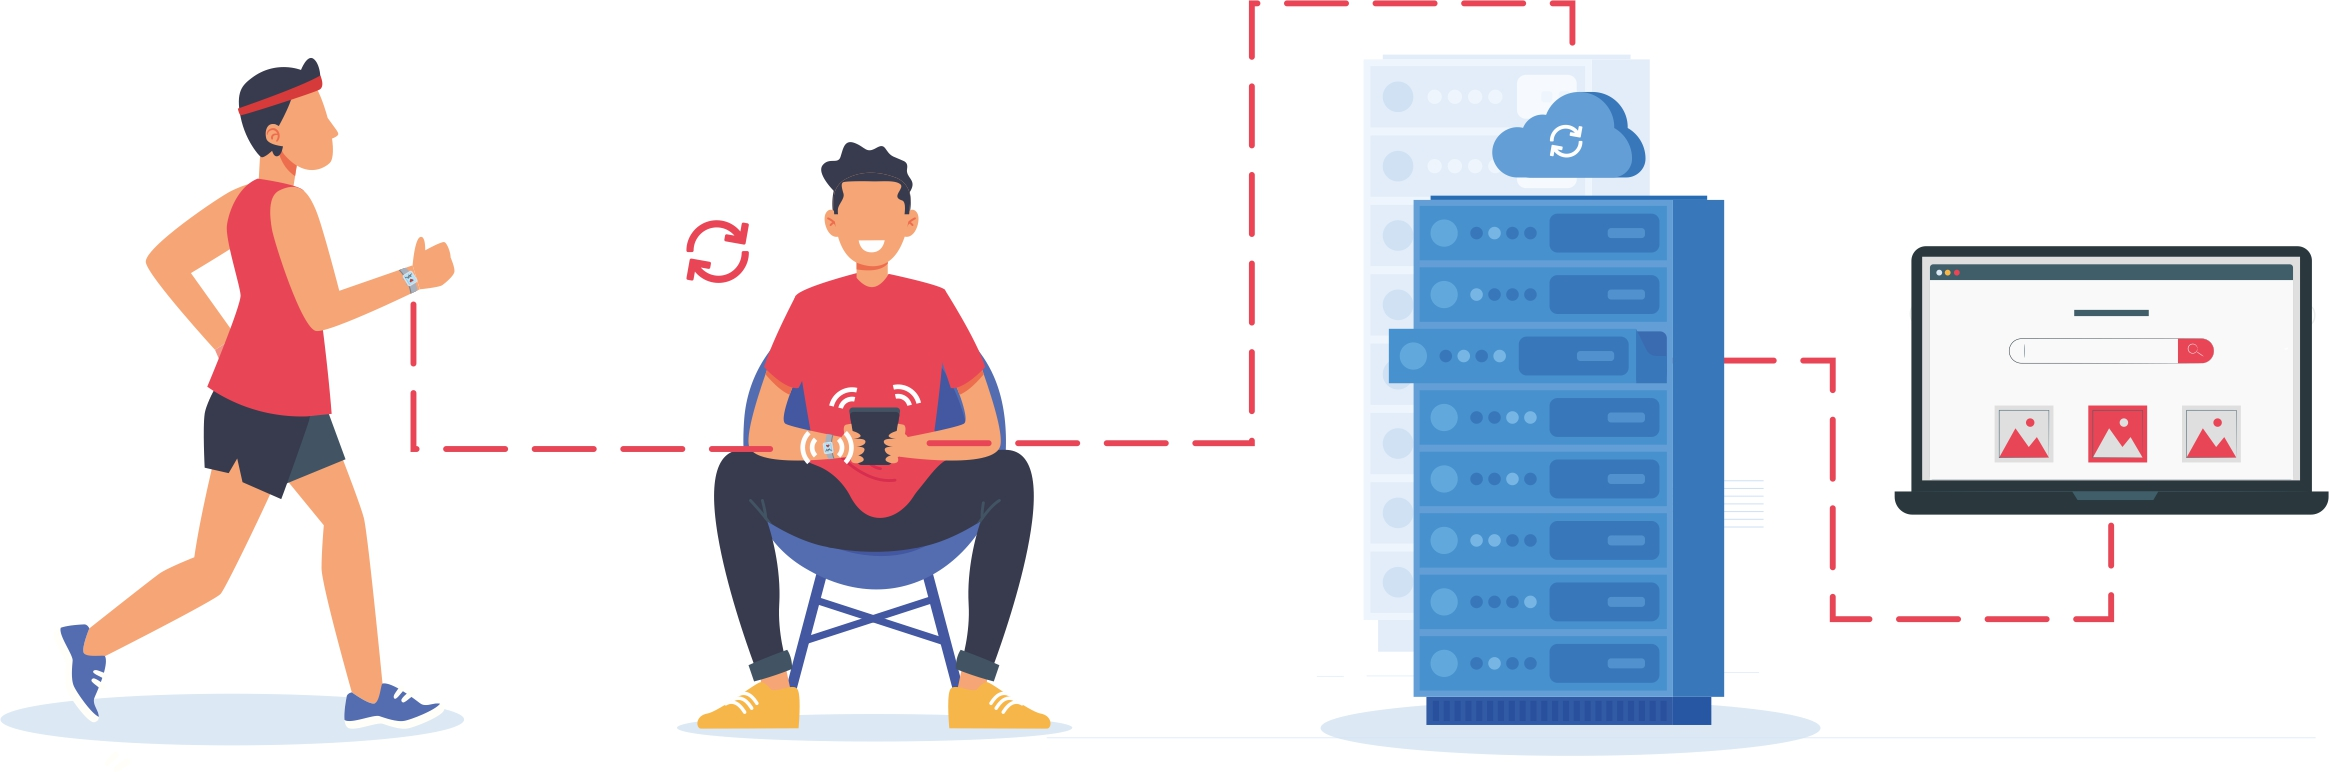
\includegraphics[scale = .5]{png/tracker.jpg}
        \end{figure}
    }
    \only<+>{
        \begin{itemize}
            \item<4> webpages
            \item<4> social media
            \item<4> smart devices
            \item<4> digital behavioral data
            \item<4> mobile phone networks
            \item<4> goverment data
            \item <4>...
        \end{itemize}
        \action<4>{\alert{The fact that you can get the data does not mean you should.}}
    }
\end{frame}

\section{Webscraping}

\begin{frame}
    \frametitle{Webscraping}
    \only<+>{
        \begin{figure}
            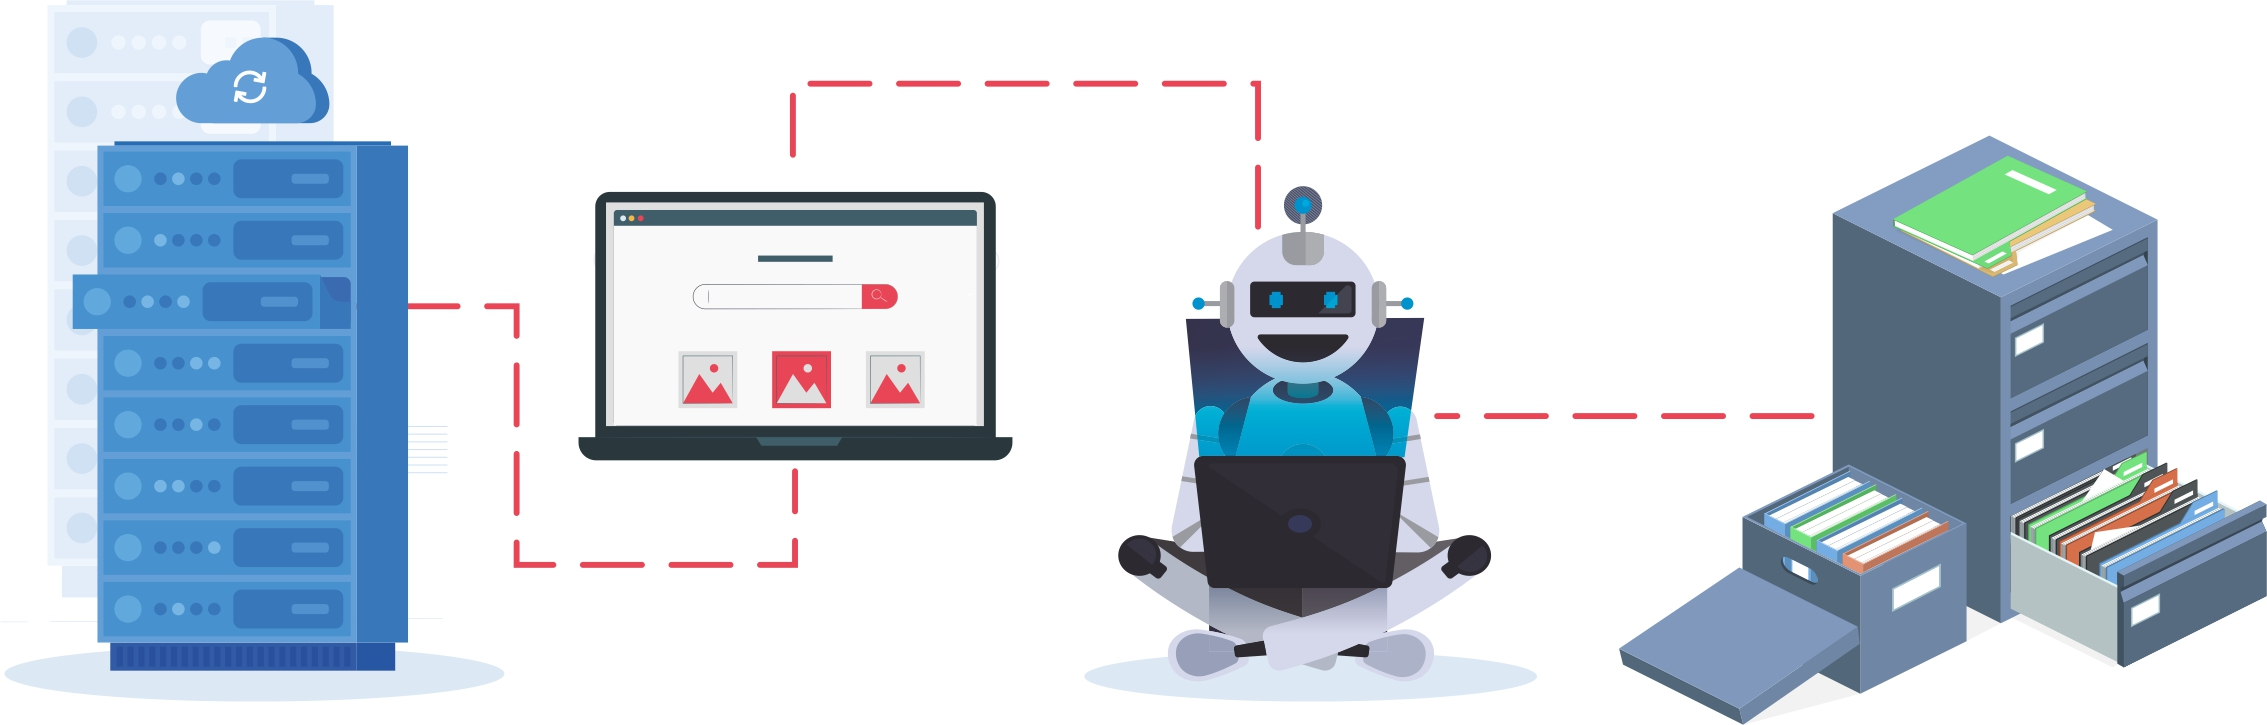
\includegraphics[scale = .5]{png/webscraping.jpg}
        \end{figure}
    }
    \only<+>{
        \begin{figure}
            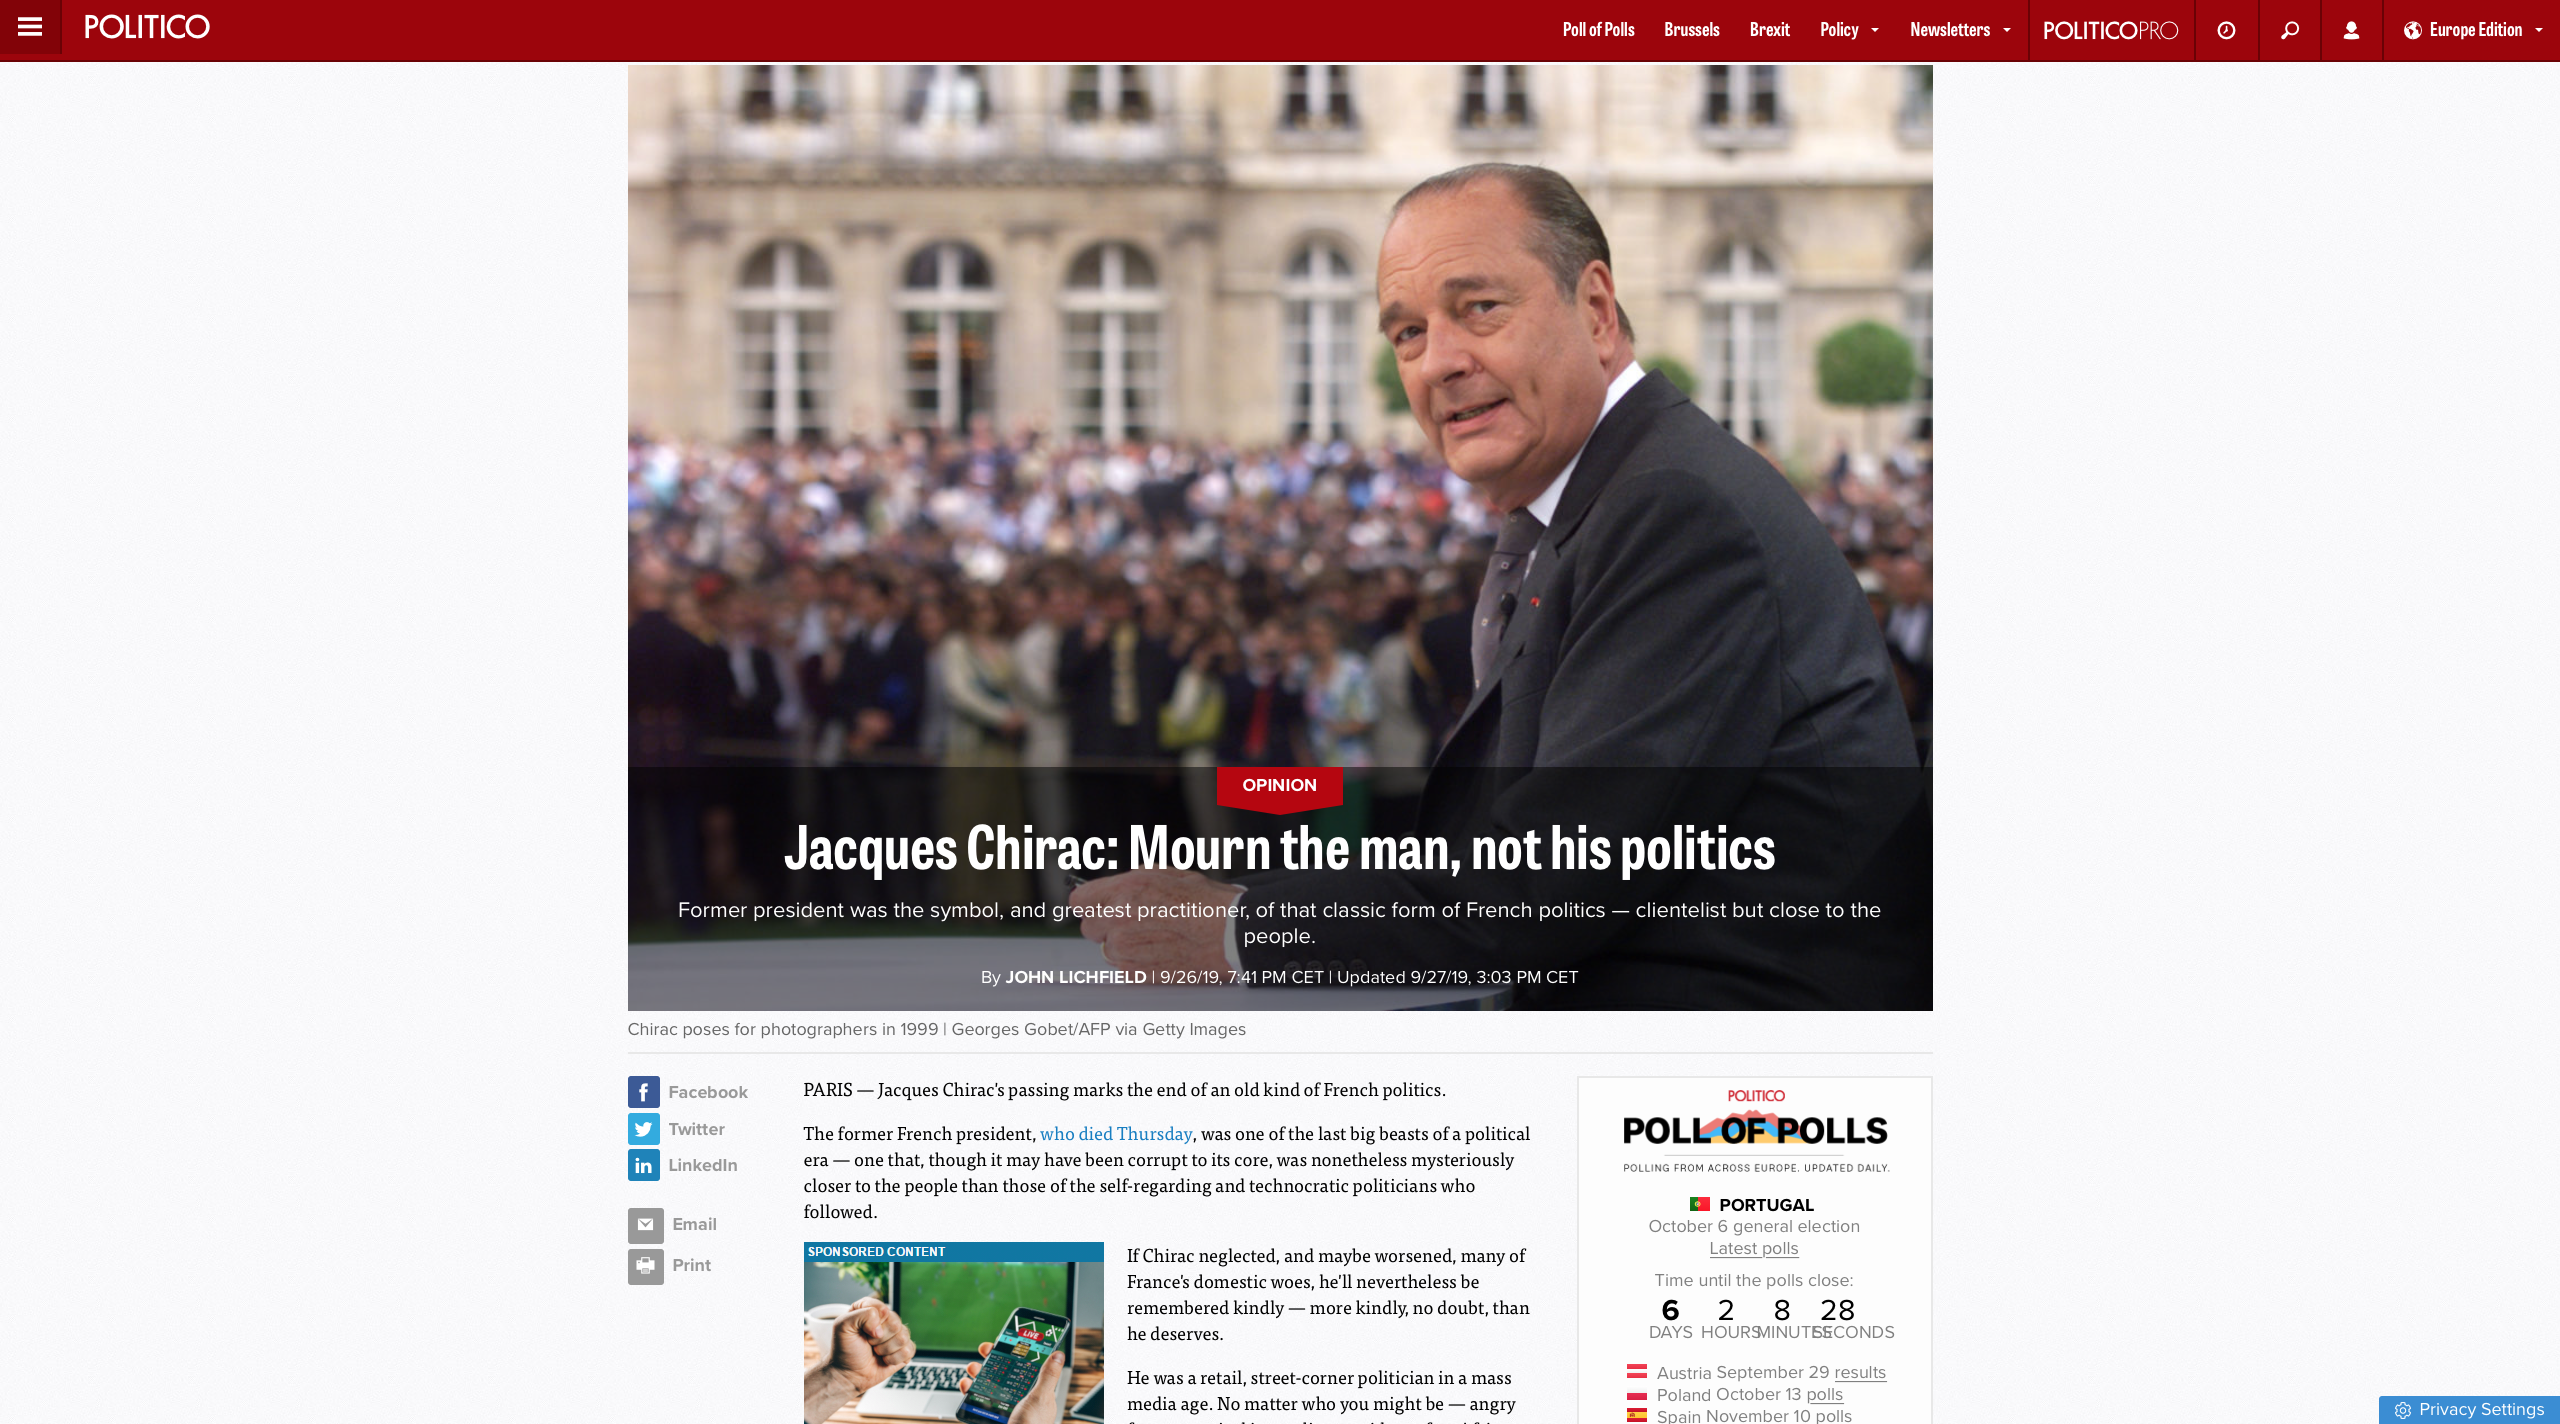
\includegraphics[scale = .22]{png/politico.png}
            \caption{from \textcolor{blue}{\href{https://www.politico.eu/article/jacques-chirac-mourn-the-man-not-his-politics/}{POLITICO Europe}}}
        \end{figure}
    }
    \only<+>{
        \begin{definition}
            \emph{Webscraping} is a process of (usually) automatic extraction of data from a website or multiple websites. In other words, it is a form of copying the data from a website into a local database or spreadsheet.
        \end{definition}
    }
\end{frame}

\subsection{HTML}

\begin{frame}
    \frametitle{HyperText Markup Language}
    \begin{definition}{}
        \emph{HyperText Markup Language} (HTML) is the standard markup language for
        documents designed to be displayed in a web browser. It defines the
        content and structure of web content. It is often assisted by
        technologies such as Cascading Style Sheets (CSS) and scripting
        languages such as JavaScript.
    \end{definition}
\end{frame}

\begin{frame}[fragile]
\frametitle{HyperText Markup Language}
\begin{minted}[fontsize=\footnotesize]{html}
<!DOCTYPE html>
<html>
    <head>
        <title>
            Justyna Kowalczyk fandom
        </title>
    </head>
    <body>
        <h1>Why Justyna Kowalczyk is the best?</h1>
        <p>
            Because she is just <b>the best</b> cross-country 
            skier in the history of the sport. You can learn
            more about her amazing achievements visiting
            her Wikipedia webpage:
            https://pl.wikipedia.org/wiki/Justyna_Kowalczyk.
        </p>
    </body>
</html>
\end{minted}
\end{frame}

\begin{frame}
    \frametitle{HyperText Markup Language}
    \only<+>{
        \framesubtitle{What are tags?}
        Tags are used to mark up the start of an HTML element and they are enclosed
        in \textbf{angle brackets}. The most important is the <html> tag. Inside
        this tag, between <html> and </html> all other elements live. In the 
        example from the previous slide we had the following tags:
        \begin{itemize}
            \item {<head></head>} -- element contains meta-information about the document
            \item {<title></title>} -- element specifies a title for the document
            \item {<body></body>} -- element contains the visible page content
            \item {<h1></h1>} -- element defines a large heading
            \item {<p></p>} -- element define a paragraph
            \item {<b></b>} -- element define a boldface
        \end{itemize}
    }
\end{frame}

\section{API}

\begin{frame}
    \frametitle{Application Programming Interface}
    \only<+>{
        \begin{figure}
            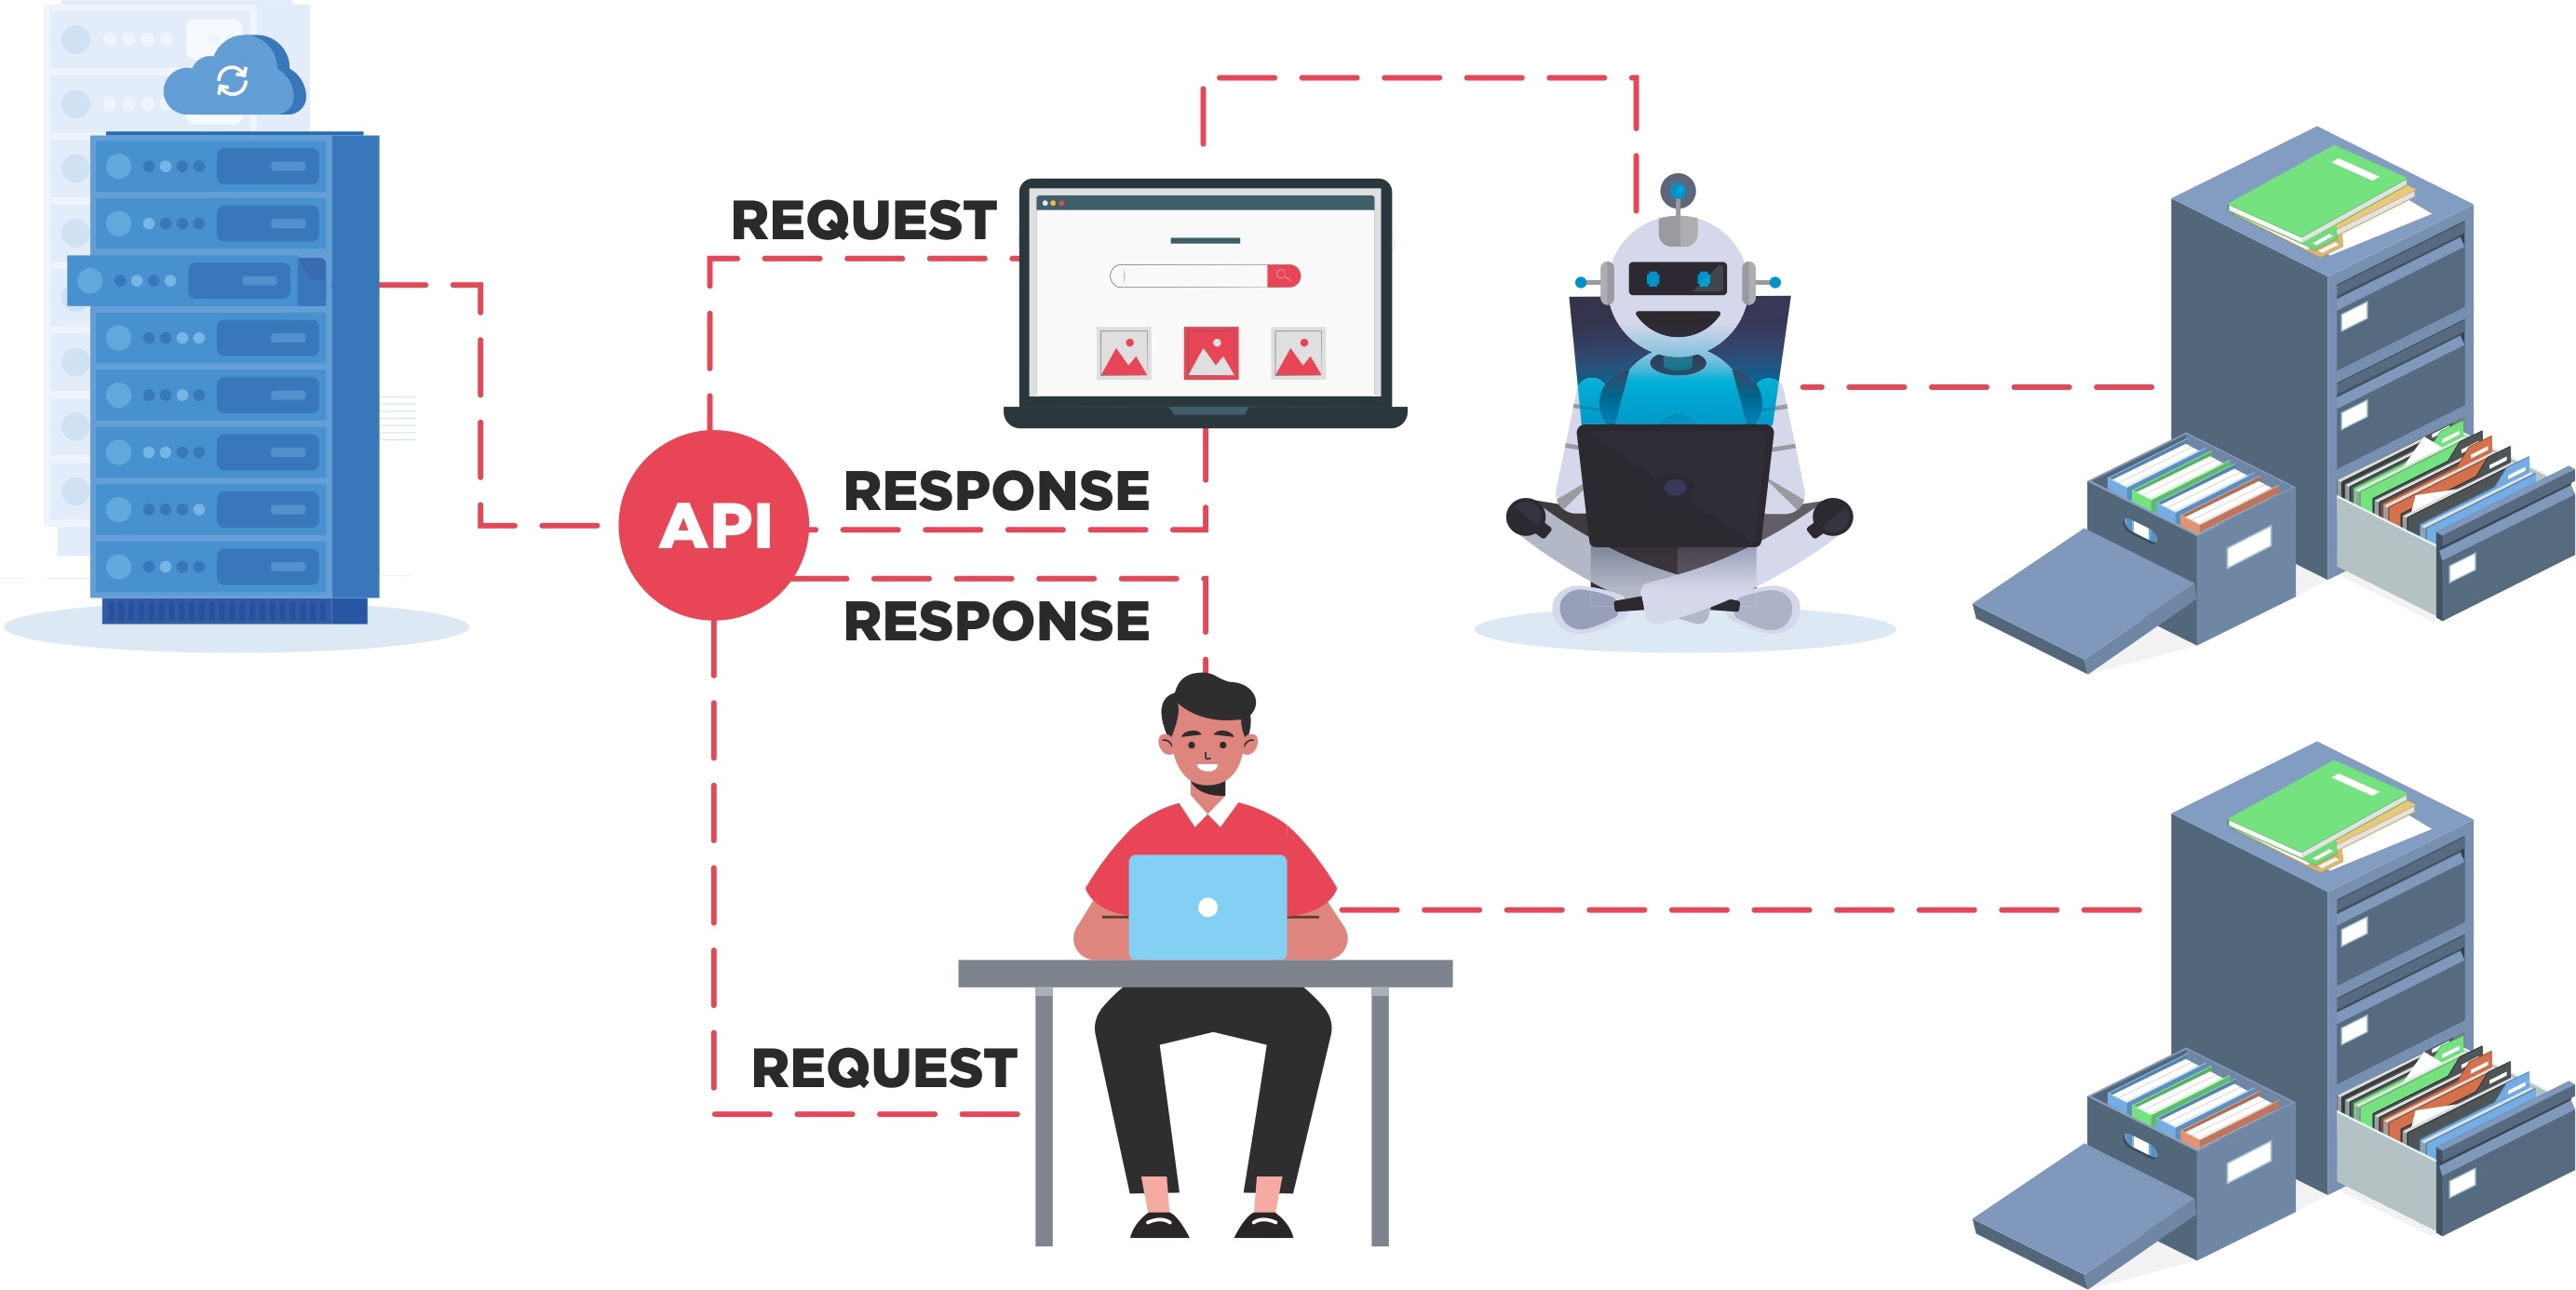
\includegraphics[scale = .4]{png/api.jpg}
        \end{figure}
    }
    \only<+>{
        \begin{figure}
            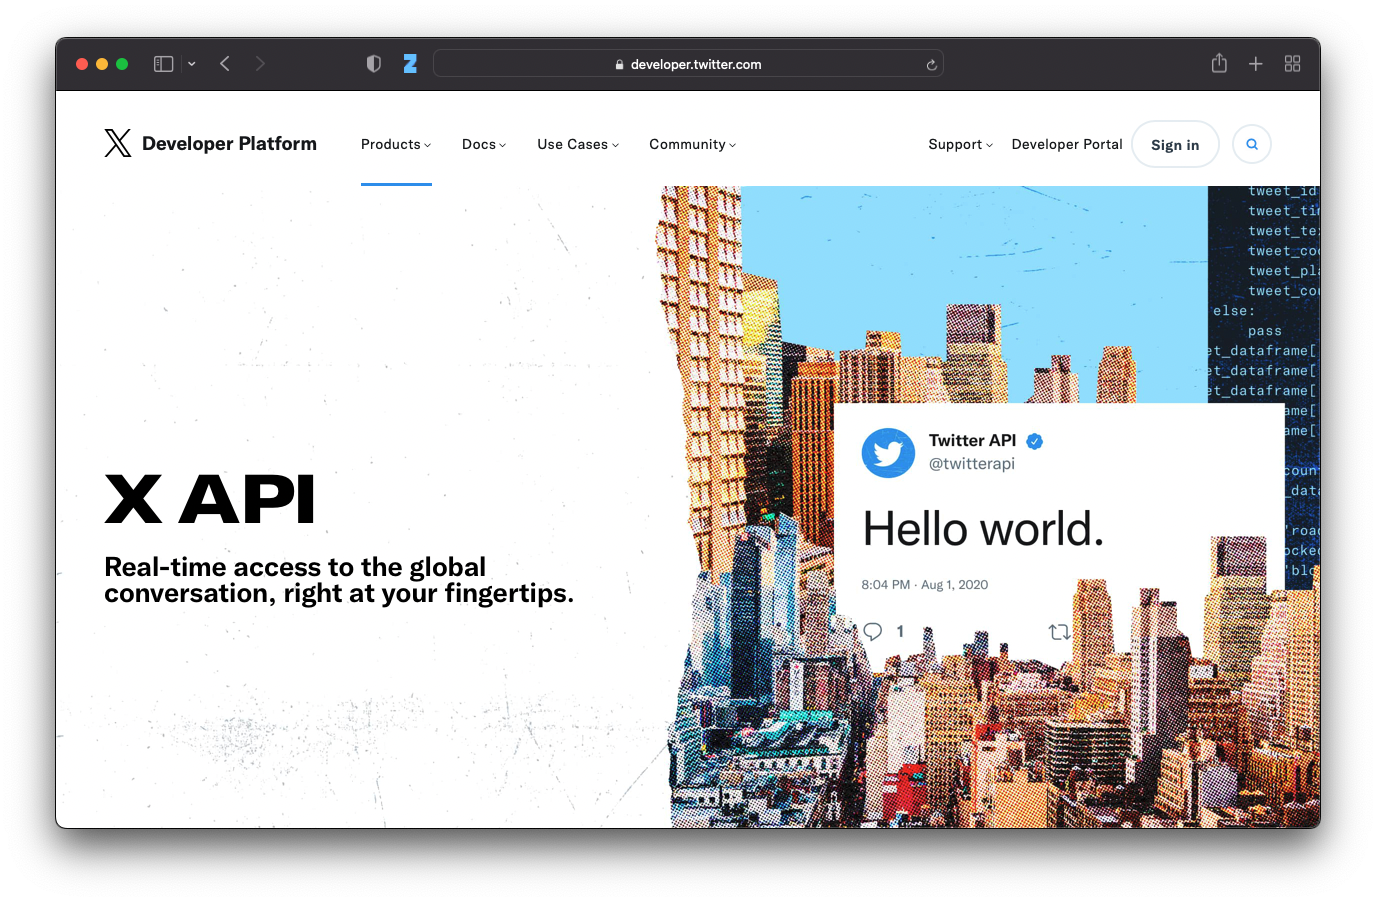
\includegraphics[width = \textwidth]{png/twitter.png}
            \caption{from \textcolor{blue}{\href{https://developer.twitter.com/en/use-cases/analyze}{Developer X}}}
        \end{figure}
    }
    \only<+>{
        \begin{definition}
            \emph{Aplication Programming Interface} is a communication protocol between a client and a server intended to simplify the building of client-side software. In other words, it is a contract between the client and the server which defines the format of possible requests and the format of the response (i.e. format of the data).
        \end{definition}
    }
\end{frame}

\section{Migrations 2.0}

\begin{frame}
    \frametitle{Measuring Migrations 2.0}
    \begin{figure}
        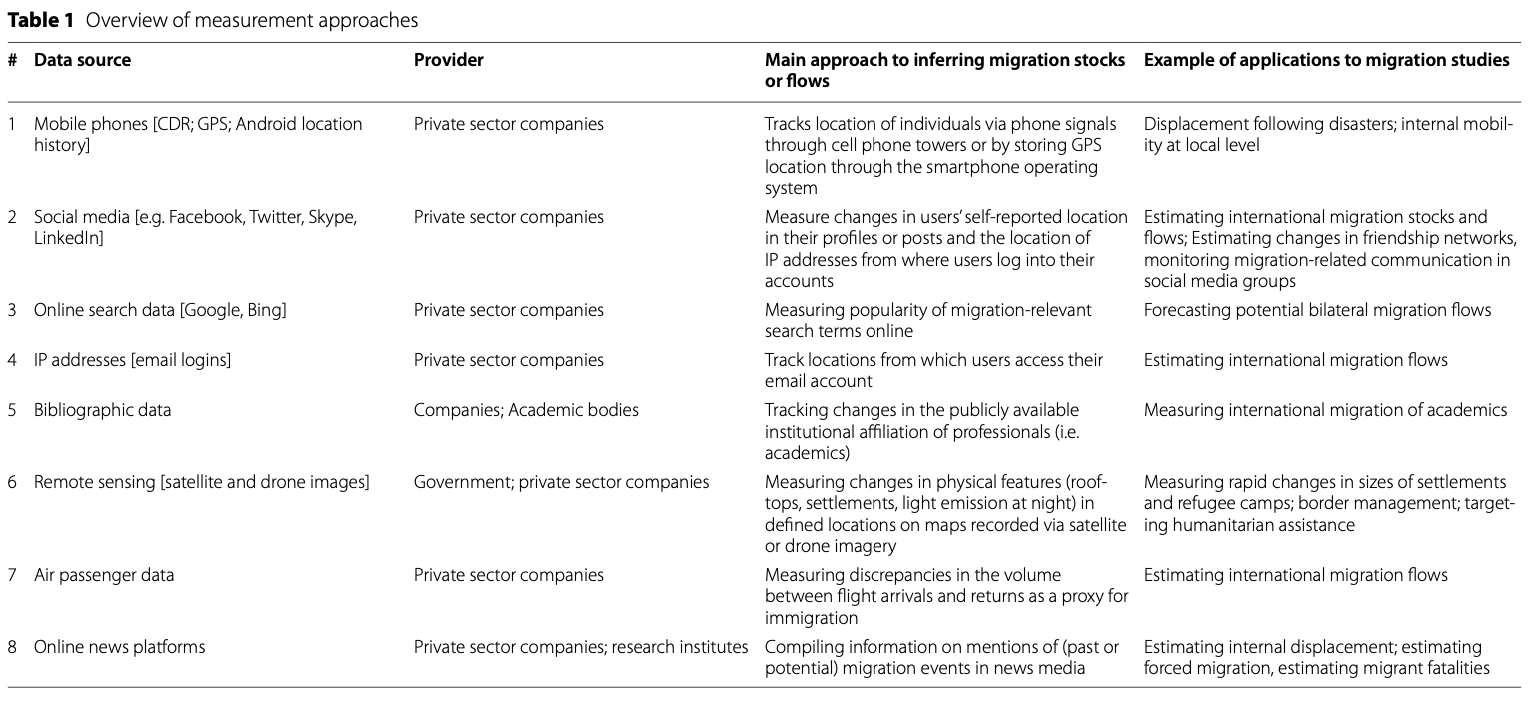
\includegraphics[width = \textwidth]{png/table.png}
        \caption{Tjaden, 2021}
    \end{figure}
\end{frame}

\begin{frame}
    \frametitle{For the class in two weeks}
    \begin{itemize}
        \item Carley, K. (1994). Extracting culture through textual analysis. Poetics, 22(4), \textcolor{red}{291–295}. \href{https://doi.org/10.1016/0304-422X(94)90011-6}{\textcolor{blue}{https://doi.org/10.1016/0304-422X(94)90011-6}}
        \item Grimmer, J., \& Stewart, B. M. (2013). Text as Data: The Promise and Pitfalls of Automatic Content Analysis Methods for Political Texts. Political Analysis, 21(3), \textcolor{red}{1-7}. \href{https://doi.org/10.1093/pan/mps028}{\textcolor{blue}{https://doi.org/10.1093/pan/mps028}}
    \end{itemize}
\end{frame}

\end{document}
